\documentclass[compress,mathserif]{beamer}
\usepackage{beamerthemesplit_z}
\usepackage{bm,bbm,graphicx}
\usepackage[czech]{babel}
\usepackage{pgf,pgfarrows,pgfnodes,pgfautomata,pgfheaps}
\usepackage{yhmath,amsmath,amssymb,amsbsy}
\usepackage[utf8]{inputenc}
\usepackage[style=german]{csquotes}
\usepackage{comment}
\hypersetup{%
  pdftitle={Náhodné veličiny a vektory},%
  pdfauthor={Lenka Křivánková}}

\title[Náhodné veličiny a vektory]{Náhodné veličiny a vektory}
\author{Lenka Křivánková}
\institute{142474@mail.muni.cz}
\date{}


\usetemplatetocsection
%{\color{structure}\inserttocsection}
{\color{structure}\insertsection}


\begin{document}

\frame{\titlepage
\begin{center}

	{Přednáška Statistika 1 (BKMSTAI)\\[5mm] 4. listopad 2016, Brno}
\end{center}}


\frame {
  \frametitle{Motivace}
  \begin{itemize}
\item Aparát vybudovaný na základě pravděpodobnosti se více formalizuje pomocí funkcí, které\\[2mm]
\begin{itemize}
	\item slouží jako teoretický model chování náhodné veličiny a \\[2mm]
	\item umožňují vyčíslit teoretické vlastnosti náhodné veličiny.\\[5mm]
\end{itemize}

\item Tyto funkce, \enquote{rozdělení} náhodných veličin, lze transformovat pro různě upravené náhodné veličiny. \\[5mm]

\item S \enquote{rozdělením} souvisí pojem kvantilů, pomocí kterých se testují hypotézy o parametrech těchto \enquote{rozdělení}.

\end{itemize}
}

\frame {
  \frametitle{Náhodná veličina}
  \begin{itemize}
	\item   {\bf Náhodnou veličinu $X$} definujeme jako zobrazení $X: \Omega \mapsto R$, kde každý vzor je jevem a obraz $X(\omega)$ se nazývá číselná realizace. Obvykle se zapisuje jen symbolem $X$. \\[4mm]
  \item Zavedení náhodné veličiny slouží zejména ke zkrácení a zpřehlednění zápisu pravděpodobností. Např. pravděpodobnost, že se náhodná veličina $X$ realizuje v~množině $B$ zkrátíme
  $$P(\{\omega\in \Omega:X(\omega)\in B\}) \Rightarrow P(X\in B)$$
  a
  $$P(\{\omega\in \Omega:X(\omega)\in B, B=(-\infty,x]\}) \Rightarrow P(X\leq x).$$
  
 \end{itemize} 
}





\frame {
  \frametitle{Distribuční funkce}
  Funkce $F: \mathbb{R}\mapsto \mathbb{R}$ definovaná vztahem 
  $$
  \forall x\in \mathbb{R}: F(x) = P(X\leq x)
  $$ 
  se nazývá {\bf distribuční funkce} náhodné veličiny $X$. Tato funkce má následující vlastnosti: 
  \begin{itemize}
	\item je neklesající, tj. pro všechna $x_1<x_2$ je $F(x_1)\leq F(x_2)$,
	\item je zprava spojitá, tj pro všechna $x_0\in \mathbb{R}$: $\lim\limits_{x\rightarrow x_0^+}F(x)=F(x_0)$,
	\item $\lim\limits_{x\rightarrow\infty}F(x)=1$, $\lim\limits_{x\rightarrow -\infty}F(x)=0$,
	\item $0\leq F(x)\leq 1$,
	\item pro $x_0\in \mathbb{R}$ libovolné, ale pevně zvolené je $P(X=x_0) = F(x_0) - \lim\limits_{x\rightarrow x_0^-}F(x)$,
	\item pro $a, b \in \mathbb{R}$, $a<b$ je $P(a<X\leq b)=F(b)-F(a)$.
\end{itemize}
  
  
}


\frame {
  \frametitle{Distribuční funkce -- příklad}
  Najděte distribuční funkci náhodné veličiny $X$, která udává, jaké číslo padlo při hodu kostkou.
  $$ x \in (-\infty, 1): F(x)=P(X\leq x) =0$$
  $$ x \in [1, 2): F(x)=P(X\leq x) =1/6$$
   $$ x \in [2, 3): F(x)=P(X\leq x) =2/6$$
   $$\vdots$$
   $$ x \in [6, \infty): F(x)=P(X\leq x) =1$$
   }

\frame {
  \frametitle{Distribuční funkce -- příklad}
  
   \begin{center}
   \scalebox{0.5}{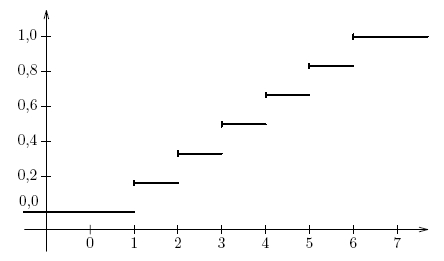
\includegraphics{03cdf.jpg}}
   \end{center}
}
\frame {
  \frametitle{Distribuční funkce -- příklad}
  
   \begin{center}
   \scalebox{0.5}{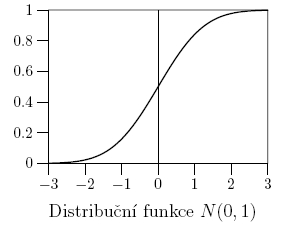
\includegraphics{03cdf2.jpg}}
   \end{center}
}


\frame {
  \frametitle{Pravděpodobnostní funkce}
  Náhodná veličina $X$ se nazývá {\bf diskrétní}, právě když existuje funkce $p(x)$, která je
  \begin{itemize}
	\item nulová v $\mathbb{R}$ s výjimkou nejméně jednoho a nejvýše spočetně mnoha bodů,
	\item kladná ($\forall x\in \mathbb{R}: p(x)\geq 0)$,
	\item normovaná ($\sum_{x=-\infty}^\infty p(x) = 1$)
	\item a platí pro ni $\forall x \in \mathbb{R}: F(x) = \sum_{t\leq x}p(t)$.
\end{itemize}
Tato funkce se nazývá {\bf pravděpodobnostní funkce} náhodné veličiny $X$.   
}



\frame {
  \frametitle{Pravděpodobnostní funkce -- vlastnosti}
Pro pravděpodobnostní funkci náhodné veličiny $X$ platí
$$\forall x \in \mathbb{R}: p(x) = P(X=x)$$
a pro libovolný pevně daný bod $x_0 \in \mathbb{R}$
$$p(x_0)=F(x_0)-\lim_{x\rightarrow x_0^-} F(x).$$
Distribuční funkce diskrétní náhodné veličiny má schodovitý charakter.
  
}




\frame {
  \frametitle{Pravděpodobnostní funkce -- příklad}
   \begin{center}
   \scalebox{0.5}{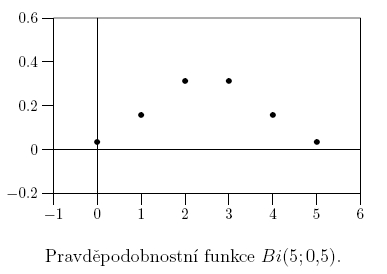
\includegraphics{03pf.jpg}}
   \end{center}  
}



\frame {
  \frametitle{Hustota}
  Náhodná veličina $X$ se nazývá {\bf spojitá}, právě když existuje po částech spojitá funkce, která je
  \begin{itemize}
	\item nezáporná ($\forall x\in \mathbb{R}: f(x)\geq 0)$,
	\item normovaná ($\int_{-\infty}^\infty f(x) dx = 1$),
	\item platí $$\forall x \in \mathbb{R}: F(x) = \int_{-\infty}^x f(t) dt, $$
	\item	$\forall B\subseteq\mathbb R:\, P(X\in B)=\int\limits_{x\in B}\varphi(x)\,dx$.
\end{itemize}
Funkce $f(x)$ se nazývá {\bf hustota pravděpodobnosti} spojité náhodné veličiny $X$. Má i následující vlastnost: 
$$f(x) = \frac{\partial F(x)}{\partial x}.$$
Distribuční funkce spojité náhodné veličiny je všude spojitá.

 
}


\frame {
  \frametitle{Hustota -- příklad}
   \begin{center}
   \scalebox{0.45}{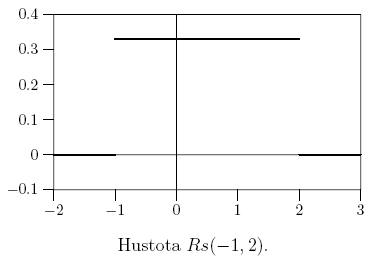
\includegraphics{03h1.jpg}}
   \scalebox{0.45}{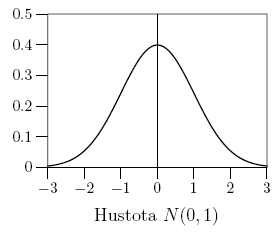
\includegraphics{03h2.jpg}}
   \end{center} 
 
}





\frame {
  \frametitle{Hustota -- příklad 1}
 $$\varphi(x)=\left\{\begin{array}{ll} k~& \mbox{pro }x\in(980,1020), \\ 0 & \mbox{jinak.}\end{array}\right.$$
Z~normovanosti hustoty plyne: $1=\int\limits_{980}^{1020}k\,dx=40k$, tedy $k=\frac1{40}$. Pro distribuční funkci platí:
 $$\Phi(x)=\left\{\begin{array}{ll}0&\mbox{pro }x\leq980, \\ \int\limits_{980}^x\frac1{40}\,dt=\frac{x-980}{40} & \mbox{pro }980<x<1020,\\1 & \mbox{pro }x\geq1020.\end{array}\right.  $$ 
}




\frame {
  \frametitle{Hustota -- příklad 2}
Doba (v~minutách) potřebná k~obsloužení zákazníka v~prodejně potravin je náhodná veličina, která se řídí rozložením $Ex(\frac13)$. Jaká je pravděpodobnost, že doba potřebná k~obsloužení náhodně vybraného zákazníka v~této prodejně bude v~rozmezí od 3 do 6 minut?
}




\frame {
  \frametitle{Hustota -- příklad 2}
$X$ -- doba potřebná k~obsloužení náhodně vybraného zákazníka, $X\sim Ex(\frac13)$, 
$$
\varphi(x)=\left\{\begin{array}{ll} \frac13e^{-\frac x3} & \mbox{pro }x>0,\\[1mm] 0 & \mbox{jinak.} \end{array}\right. $$
\begin{eqnarray*}
	 P(3\leq X \leq6)&=&\int\limits_3^6\frac13 e^{-\frac x3}\,dx\\
	 &=&\frac13(-3)\left[e^{-\frac x3}\right]_3^6\\
	 &=&-e^{-2}+e^{-1}=0,\!233. 
\end{eqnarray*}
}



\frame {
  \frametitle{Náhodný vektor}
  Nechť $X_1, \dots, X_n$ jsou náhodné veličiny a $F_1, \dots, F_n$ jsou jejich distribuční funkce. Pak definujeme {\bf náhodný vektor} jako uspořádanou $n$-tici $\bm{X}=(X_1, \dots, X_n)$. Jeho distribuční funkci definujeme vztahem
  $$ \forall (x_1, \dots, x_n)\in \mathbb{R}^n: F(x_1, \dots, x_n) = P(X_1\leq x_1 \wedge \dots \wedge X_n\leq x_n).$$
  
  Platí vlastnosti distribuční funkce náhodné veličiny, navíc máme
  $$\forall i\in \{1, \dots, n\}: \lim_{x_1, \dots, x_{i-1},x_{i+1},\dots, x_n \rightarrow\infty} F(x_1, \dots, x_n) = F_i(x_i),$$
  
 kde $F_i(x_i)$ se v této souvislosti nazývá marginální distribuční funkce náhodné veličiny $X_i$ a $F(x_1, \dots, x_n)$ se nazývá simultánní distribuční funkce náhodného vektoru $\bm{X}$. 
  
  
}

\frame {
  \frametitle{Diskrétní náhodný vektor}
  Náhodný vektor $\bm{X}$ se nazývá diskrétní, právě když existuje funkce $p(x_1, \dots, x_n)$, která je
  \begin{itemize}
	\item nulová v $\mathbb{R}^n$ s výjimkou nejméně jednoho a nejvýše spočetně mnoha bodů,
	\item kladná
	\item normovaná ($\sum_{x_1=-\infty}^\infty \cdots \sum_{x_n=-\infty}^\infty p(x_1, \dots, x_n) = 1$)
	\item a platí pro ni
	$$
\forall (x_1, \dots, x_n)\in \mathbb{R}^n: F(x_1, \dots, x_n) = \sum_{t_1\leq x_1} \cdots \sum_{t_n\leq x_n} p(t_1, \dots, t_n).
	$$
	\end{itemize}
	Funkce $p(x_1, \dots, x_n)$ se nazývá pravděpodobnostní funkce diskrétního náhodného vektoru $\bm{X}$.
	 
}


\frame {
  \frametitle{Diskrétní náhodný vektor}
	Pro pravděpodobnostní funkci dále platí
	$$ \forall (x_1, \dots, x_n)\in \mathbb{R}^n: p(x_1, \dots, x_n) = P(X_1= x_1 \wedge \dots \wedge X_n= x_n)$$
	a
	$$\forall i\in \{1, \dots, n\}: \sum_{x_1\in \mathbb{R}}\cdots\sum_{x_{i-1}\in \mathbb{R}}\sum_{x_{i+1}\in \mathbb{R}}\cdots \sum_{x_n\in \mathbb{R}} p(x_1, \dots, x_n) =p_i(x_i).$$
	Funkce $p_i(x_i)$ se nazývá marginální pravděpodobnostní funkce náhodné veličiny $X_i$ a $p(x_1, \dots, x_n)$ simultánní pravděpodobnostní funkce náhodného vektoru $\bm{X}$.
	
Pravděpodobnost, že se náhodný vektor $\bm{X}$ bude realizovat v oblasti $B\subseteq \mathbb{R}^n$, se vypočte podle vzorce
$$P(\bm{X}\in B)=\sum\cdots\sum_{\hspace*{-1.1cm}(x_1, \dots, x_n)\in B} p(x_1, \dots, x_n).$$
  
  
}


\frame {
  \frametitle{Diskrétní náhodný vektor -- příklad}
  \begin{center}\hspace*{-5mm}
	\begin{tabular}{|c||c|c|c|c||c|}
\hline
\parbox[c][1cm]{15mm}{\raisebox{-2mm}{$x_1$} \quad \ \raisebox{2mm}{$x_2$}} & \parbox{15mm}{\centering 0} & \parbox{15mm}{\centering 1} & \parbox{15mm}{\centering 2} & \parbox{15mm}{\centering 3} & \parbox{15mm}{\mbox{}\hfill\mbox{}$\pi_1(x_1)$\hfill\mbox{}} \\
\hline\hline
\parbox{15mm}{\centering -1}	& $2c$ & $c$ &	0	&0	& $3c$ \\\hline
 0	& $c$	& $2c$ &	$c$	& 0	& $4c$ \\\hline
 1	& 0	& 0	& $2c$ &	$c$	& $3c$ \\\hline\hline
$\pi_2(x_2)$ &	$3c$	& $3c$ &	$3c$ & 	$c$	& 1 \\ \hline
\end{tabular}
\end{center}
  
}



\frame {
  \frametitle{Spojitý náhodný vektor}
  Náhodný vektor $\bm{X}$ se nazývá spojitý, právě když existuje po částech spojitá funkce $f(x_1, \dots, x_n)$, která je
  \begin{itemize}
	\item nezáporná,
	\item normovaná ($\int\limits_{-\infty}^\infty \cdots \int\limits_{-\infty}^\infty f(x_1, \dots, x_n) dx_1 \cdots dx_n = 1$)
	\item a platí pro ni
$$ 
\forall (x_1, \dots, x_n)\in \mathbb{R}^n:F(x_1, \dots, x_n) =
$$
$$
= \int_{-\infty}^{x_1} \cdots \int_{-\infty}^{x_n} f(t_1, \dots, t_n) dt_1 \cdots dt_n.
$$
\end{itemize}
  Funkce $f(x_1, \dots, x_n)$ se nazývá {\bf hustota pravděpodobosti} spojitého náhodného vektoru $\bm{X}$.
  
}

\frame {
  \frametitle{Hustota spojitého náhodného vektoru}
  Pro hustotu pravděpodobnosti spojitého náhodného vektoru $\bm{X}$ dále platí
  $$ f(x_1, \dots, x_n)=\frac{\partial^nF(x_1, \dots, x_n)}{\partial x_1 \cdots \partial x_n}$$
  a $\forall i\in \{1, \dots, n\}$: 
  $$\int\limits_{-\infty}^\infty \cdots \int\limits_{-\infty}^\infty \int\limits_{-\infty}^\infty \cdots \int\limits_{-\infty}^\infty f(x_1, \dots, x_n) dx_1 \cdots dx_{i-1} dx_{i+1} \cdots dx_n = f_i(x_i).$$
  Funkce $f_i(x_i)$ se nazývá marginální hustota náhodné veličiny $X_i$ a $f(x_1, \dots, x_n)$ se nazývá simultánní hustota náhodného vektoru $\bm{X}$.
  
  Pravděpodobnost, že se náhodný vektor $\bm{X}$ bude realizovat na oblasti $B\subseteq \mathbb{R}^n$ je rovna
  $$
  P(\bm{X}\in B)=\int\cdots\int_{B}f(x_1, \dots, x_n) dx_1 \cdots dx_n .$$
  
}

\frame {
  \frametitle{Hustota spojitého náhodného vektoru -- příklad}
     \begin{center}
   \scalebox{0.5}{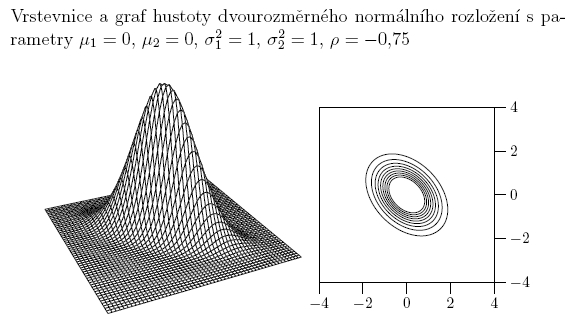
\includegraphics{03nvh.jpg}}
   \end{center} 
}


\frame {
  \frametitle{Stochastická nezávislost náhodných veličin}
  Náhodné veličiny $X_1, \dots, X_n$ jsou stochasticky nezávislé právě tehdy, když pro každé $x_1\in \mathbb{R}, \dots, x_n\in \mathbb{R}$ platí
  $$F(x_1, \dots, x_n)=F_1(x_1)\cdot\cdots\cdot F_n(x_n),$$
  respektive
  $$ p(x_1, \dots, x_n)=p_1(x_1)\cdot\cdots\cdot p_n(x_n)$$
  v diskrétním případě nebo
  $$ f(x_1, \dots, x_n)=f_1(x_1)\cdot\cdots\cdot f_n(x_n)$$
  ve spojitém případě.
  
}

\frame {
  \frametitle{Stochastická nezávislost náhodných veličin -- příklad}
Náhodný vektor $(X_1,X_2)$ má pravděpodobnostní funkci danou následující tabulkou. 

Zjistěte, zda jsou náhodné veličiny stochasticky nezávislé či nikoliv.\\[1cm]

\begin{overprint}

\onslide<1>

\begin{center}
	\begin{tabular}{c|cc}
	\multicolumn{1}{c}{\ }&\multicolumn{2}{c}{$X_2$}\\
	$X_1$&0&1\\ \hline
	-1&1/3&0\\
	0&0&1/3\\
	1&1/3&0\\
	\end{tabular}
	\end{center}
	
\onslide<2>

\begin{center}
	\begin{tabular}{c|cc|c}
	\multicolumn{1}{c}{\ }&\multicolumn{2}{c}{$X_2$}\\
	$X_1$&0&1&$p_1(x_1)$\\ \hline
	-1&1/3&0&1/3\\
	0&0&1/3&1/3\\
	1&1/3&0&1/3\\ \hline
	$p_2(x_2)$&2/3&1/3&1\\
	\end{tabular}
\end{center}

\onslide<3>

\begin{center}
	\begin{tabular}{c|cc|c}
	\multicolumn{1}{c}{\ }&\multicolumn{2}{c}{$X_2$}\\
	$X_1$&0&1&$p_1(x_1)$\\ \hline
	-1&{\bf \textcolor{red}{1/3}}&0&{\bf \textcolor{red}{1/3}}\\
	0&0&1/3&1/3\\
	1&1/3&0&1/3\\ \hline
	$p_2(x_2)$&{\bf\textcolor{red}{2/3}}&1/3&1\\
	\end{tabular}\\[1cm]
	Náhodné veličiny $X_1$ a $X_2$ {\bf nejsou} stochasticky nezávislé.
\end{center}
\end{overprint}	

}

\frame {
  \frametitle{Transformované náhodné veličiny a vektory}
  Nechť $g$ je vhodná funkce (nejčastěji spojitá). Pak můžeme pomocí této funkce transformovat náhodnou veličinu $X$ na (transformovanou) náhodnou veličinu $Y$. Formálně píšeme
  $$
  \forall \omega \in \Omega: Y(\omega) = g(X(\omega)).
  $$
  Stejně tak můžeme pomocí vhodné funkce $h$ transformovat náhodný vektor $\bm{X}$ na transformovaný náhodný vektor $\bm{Y}$ nebo na transformovanou náhodnou veličinu $Y$.
  
\begin{itemize}
	\item Pomocí transformací normálně rozdělených veličin se sestrojují veličiny pomocí nichž se testují hypotézy.
	\item {\bf Při analýze nelze data libovolně transformovat. Většinou se tím změní jejich rozdělení a získané výsledky budou nesmyslné.}
\end{itemize}  
  
}

\frame {
  \frametitle{Transformovaný náhodný vektor -- příklad}
 Předpokládejme, že doba čekání zákazníka před pokladnou je náhodná veličina, která se řídí exponenciálním rozdělením s parametrem $\lambda$. Náhodně vybereme $n$ zákazníků. Jaká je pravděpodobnost, že nejdéle čekající zákazník čekal méně než $y$ sekund?
 
Exponenciální rozdělení má hustotu
$$f(x_i)=\left\{
\begin{array}{cl}
\lambda e^{-\lambda x_i}& \mathrm{pro\ } x_i > 0, \lambda > 0\\
0& \mathrm{jinak}\\
\end{array}
\right. \quad i=1, \dots, n$$
a distribuční funkci
$$F(x_i)=\left\{
\begin{array}{cl}
1-e^{-\lambda x_i}& \mathrm{pro\ } x_i > 0\\
0& \mathrm{pro\ } x_i\leq 0\\
\end{array}
\right. \quad i=1, \dots, n.$$

Hledáme vlastně rozdělení transformované náhodné veličiny $$Y = \max\{X_1, \dots, X_n\}.$$

 
  
}

\frame {
  \frametitle{Transformovaný náhodný vektor -- příklad}

 $$F_Y(y)=P(Y\leq y)=P(\max\{X_1, \dots, X_n\}\leq y)=$$
 %$$=P(X_1\leq y \wedge \cdots \wedge X_n\leq y)=P(X_1\leq y) \cdots P(X_n\leq y)= $$
 $$=P(X_1\leq y \wedge \cdots \wedge X_n\leq y)=P(X_1\leq y) \cdot \ldots \cdot P(X_n\leq y)= $$
 %$$=F_X(y)\cdots F_X(y)=[F_X(y)]^n=(1-e^{-\lambda y})^n$$
 $$=F_X(y)\cdot \ldots \cdot F_X(y)=[F_X(y)]^n=(1-e^{-\lambda y})^n$$
 \begin{center}
 Nejdéle čekající zákazník nečekal déle než $y$ sekund s~pravděpodobností  $(1-e^{-\lambda y})^n$.
  \end{center}
}

\begin{comment}
\frame {
  \frametitle{Podmíněná distribuční funkce}
  \begin{itemize}
	\item Nechť $(X_1, X_2)$ je náhodný vektor se simultánní distribuční funkcí $\Phi \left(x_{1} ,x_{2}  \right)$.\\[2mm]
	
	\item Podmíněná distribuční funkce $\Phi _{1\left|2\right. } \left(x_{1} \left|{ x}_{{ 2}} \right. \right)$ náhodné veličiny $X_1$ za podmínky, že náhodná veličina $X_2$ nabývá hodnoty $x_2$, je dána vztahem
$$
\forall x_{1} \in \mathbb R:\Phi _{1\left|2\right. } \left(x_{1} \left|x_{2} \right. \right)
$$
$$
=\lim _{\Delta x_{2} \to 0} P\left(X_{1} \le x_{1} \left|x_{2} <X_{2} \le x_{2} +\Delta x_{2} \right. \right) 
$$
$$
=\lim _{\Delta x_{2} \to 0} \frac{P\left(X_{1} \le x_{1} \wedge x_{2} <X_{2} \le x_{2} +\Delta x_{2} \right)}{P\left(x_{2} <X_{2} \le x_{2} +\Delta x_{2} \right)}. 
$$\\[2mm]
\item Analogicky lze definovat podmíněnou distribuční funkci $\Phi _{2\left|1\right. } \left(x_{2} \left|x_{1} \right. \right)$.
\end{itemize}
 


}


\frame {
  \frametitle{Podmíněná distribuční funkce}

 Nechť $(X_1, X_2)$ je náhodný vektor s~marginálními distribučními funkcemi $\Phi _{1} \left(x_{1} \right)$ a~$\Phi _{2} \left(x_{2} \right)$. Náhodné veličiny $X_1$, $X_2$ jsou stochasticky nezávislé, jestliže platí:
$$
\forall x_{2} \in \mathbb R:\Phi _{1\left|2\right. } \left(x_{1} \left|x_{2} \right. \right)=\Phi _{1} \left(x_{1} \right)
$$ 
a současně 
$$
\forall x_{1} \in \mathbb R:\Phi _{2\left|1\right. } \left(x_{2} \left|x_{1} \right. \right)=\Phi _{2} \left(x_{2} \right).
$$

}


\frame {
  \frametitle{Podmíněná pravděpodobnostní funkce}

\begin{itemize}
	\item Nechť $(X_1, X_2)$ je diskrétní náhodný vektor se simultánní pravděpodobnostní funkcí $\pi \left(x_{1} ,x_{2} \right)$ a marginálními pravděpodobnostními funkcemi $\pi _{1} \left(x_{1} \right)$ a $\pi _{2} \left(x_{2} \right)$.\\[2mm]
	\item Fixujeme hodnotu $x_2$.\\[2mm]
	\item Podmíněná pravděpodobnostní funkce $\pi _{1\left|2\right. } \left(x_{1} \left|x_{2} \right. \right)$ náhodné veličiny $X_1$ za podmínky, že náhodná veličina $X_2$ nabývá hodnoty $x_2$, je dána vztahem
$$
\forall x_{1} \in \mathbb{R}:\pi _{1\left|2\right. } \left(x_{1} \left|x_{2} \right. \right)=\frac{\pi \left(x_{1} ,x_{2} \right)}{\pi _{2} \left(x_{2} \right)} {\mathrm {\; pro\;} }\pi _{2} \left(x_{2} \right)>0.
$$ 
	\item Analogicky lze definovat podmíněnou pravděpodobnostní  funkci $\pi _{2\left|1\right. } \left(x_{2} \left|x_{1} \right. \right)$.
\end{itemize}
  



}


\frame {
  \frametitle{Podmíněná pravděpodobnostní funkce}

Z~definičního vztahu je okamžitě vidět: 
 $$
 \pi \left(x_{1} ,x_{2} \right)=\pi _{2} \left(x_{2} \right)\pi _{1\left|2\right. } \left(x_{1} \left|x_{2} \right. \right),
$$ 
jestliže $\pi _{2} \left(x_{2} \right)>0$, a obdobně 
$$
\pi \left(x_{1} ,x_{2} \right)=\pi _{1} \left(x_{1} \right)\pi _{2\left|1\right. } \left(x_{2} \left|x_{1} \right. \right),
$$ 
jestliže $\pi _{1} \left(x_{1} \right)>0$. Z~těchto dvou vztahů vyplývá, že 
$$
\pi _{2\left|1\right. } \left(x_{2} \left|x_{1} \right. \right)=\frac{\pi _{1\left|2\right. } \left(x_{1} \left|x_{2} \right. \right)\pi _{2} \left(x_{2} \right)}{\pi _{1} \left(x_{1} \right)} 
$$ 
a podobně 
$$
\pi _{1\left|2\right. } \left(x_{1} \left|x_{2} \right. \right)=\frac{\pi _{2\left|1\right. } \left(x_{2} \left|x_{1} \right. \right)\pi _{1} \left(x_{1} \right)}{\pi _{2} \left(x_{2} \right)}. 
$$ 
Jedná se o Bayesův vzorec pro diskrétní náhodný vektor $(X_1, X_2)$.


}


\frame {
  \frametitle{Podmíněná distribuční funkce}


Je-li $(X_1, X_2)$ diskrétní náhodný vektor, pak pro podmíněnou distribuční funkci $\Phi _{1\left|2\right. } \left(x_{1} \left|{ x}_{{ 2}} \right. \right)$ platí: 
$$
\forall x_{1} \in \mathbb R:\Phi _{1\left|2\right. } \left(x_{1} \left|x_{2} \right. \right)=\frac{\sum\limits _{t\le x_{1} }\pi \left(t,x_{2} \right) }{\pi _{2} \left(x_{2} \right)} {\mathrm {\; pro\;} }\pi _{2} \left(x_{2} \right)>0.
$$


}


\frame {
  \frametitle{Podmíněná pravděpodobnostní funkce}
\begin{itemize}
	\item Nechť $(X_1, X_2)$ je diskrétní náhodný vektor s~marginálními pravděpodobnostními funkcemi $\pi _{1} \left(x_{1} \right)$ a $\pi _{2} \left(x_{2} \right)$.\\[3mm]
	\item Náhodné veličiny $X_1$, $X_2$ jsou stochasticky nezávislé, jestliže platí
$$
\forall x_{2} \in \mathbb R,\pi _{2} \left(x_{2} \right)>0:\pi _{1\left|2\right. } \left(x_{1} \left|x_{2} \right. \right)=\pi _{1} \left(x_{1} \right).
$$ \\[3mm]
	\item Analogicky, náhodné veličiny $X_1$, $X_2$ jsou stochasticky nezávislé, jestliže platí 
$$
\forall x_{1} \in \mathbb R,\pi _{1} \left(x_{1} \right)>0:\pi _{2\left|1\right. } \left(x_{2} \left|x_{1} \right. \right)=\pi _{2} \left(x_{2} \right).
$$
\end{itemize}
}


\frame {
  \frametitle{Podmíněná hustota pravděpodobnosti}
\begin{itemize}
	\item Nechť $(X_1, X_2)$ je spojitý náhodný vektor se simultánní hustotou  pravděpodobnosti $\varphi \left(x_{1} ,x_{2} \right)$ a marginálními hustotami pravděpodobnosti $\varphi _{1} \left(x_{1} \right)$ a $\varphi _{2} \left(x_{2} \right)$.\\[2mm]
	\item Fixujeme hodnotu $x_2$.\\[2mm]
	\item Podmíněná hustota pravděpodobnosti $\varphi _{1\left|2\right. } \left(x_{1} \left|x_{2} \right. \right)$ náhodné veličiny $X_1$ za podmínky, že náhodná veličina $X_2$ nabývá hodnoty $x_2$, je dána vztahem
$$
\forall x_{1} \in R:\varphi _{1\left|2\right. } \left(x_{1} \left|x_{2} \right. \right)=\frac{\varphi \left(x_{1} ,x_{2} \right)}{\varphi _{2} \left(x_{2} \right)} {\mathrm {\; pro\;} }\varphi _{2} \left(x_{2} \right)>0.
$$ \\[2mm]
	\item Analogicky lze definovat podmíněnou hustotu pravděpodobnosti $\varphi _{2\left|1\right. } \left(x_{2} \left|x_{1} \right. \right)$.
\end{itemize}

}


\frame {
  \frametitle{Podmíněná hustota pravděpodobnosti}


Podobně jako v~diskrétním případě lze z~definičních vztahů pro podmíněné hustoty pravděpodobnosti odvodit Bayesův vzorec pro spojitý náhodný vektor: 
$$
\varphi _{2\left|1\right. } \left(x_{2} \left|x_{1} \right. \right)=\frac{\varphi _{1\left|2\right. } \left(x_{1} \left|x_{2} \right. \right)\varphi _{2} \left(x_{2} \right)}{\varphi _{1} \left(x_{1} \right)} 
$$ 
a analogicky 
$$
\varphi _{1\left|2\right. } \left(x_{1} \left|x_{2} \right. \right)=\frac{\varphi _{2\left|1\right. } \left(x_{2} \left|x_{1} \right. \right)\varphi _{1} \left(x_{1} \right)}{\varphi _{2} \left(x_{2} \right)}. 
$$ 

}


\frame {
  \frametitle{Podmíněná distribuční funkce}

Je-li $(X_1, X_2)$ spojitý náhodný vektor, pak pro podmíněnou distribuční funkci  $\Phi _{1\left|2\right. } \left(x_{1} \left|{ x}_{{ 2}} \right. \right)$ platí 
 $$
 \forall x_{1} \in \mathbb R:\Phi _{1\left|2\right. } \left(x_{1} \left|x_{2} \right. \right)=\frac{\int _{-\infty }^{x_1}\varphi \left(t,x_{2} \right)dt }{\varphi _{2} \left(x_{2} \right)} {\mathrm {\; pro\;} }\varphi _{2} \left(x_{2} \right)>0.
 $$
 
 }


\frame {
  \frametitle{Podmíněná hustota pravděpodobnosti}
 \begin{itemize}
	\item Nechť $(X_1, X_2)$ je spojitý náhodný vektor s~marginálními hustotami pravděpodobnosti $\varphi _{1} \left(x_{1} \right)$ a $\varphi _{2} \left(x_{2} \right)$.
	\item Náhodné veličiny $X_1$, $X_2$ jsou stochasticky nezávislé, jestliže platí 
$$
\forall x_{2} \in \mathbb R,\varphi _{2} \left(x_{2} \right)>0:\varphi _{1\left|2\right. } \left(x_{1} \left|x_{2} \right. \right)=\varphi _{1} \left(x_{1} \right).
$$ 
	\item Analogicky: Náhodné veličiny $X_1$, $X_2$ jsou stochasticky nezávislé, jestliže platí 
$$
\forall x_{1} \in \mathbb R,\varphi _{1} \left(x_{1} \right)>0:\varphi _{2\left|1\right. } \left(x_{2} \left|x_{1} \right. \right)=\varphi _{2} \left(x_{2} \right).
$$
\end{itemize}

}


\frame {
  \frametitle{Podmíněné pravděpodobnosti}
\begin{itemize}
	\item Nechť $B\subseteq \mathbb R$ a náhodná veličina $X_2$ nabývá hodnoty $x_2$.\\[4mm]
	\item Zajímá nás podmíněná pravděpodobnost $P\left(X_{1} \in B\left|X_{2} =x_{2} \right. \right)$.\\[3mm]
 
\begin{itemize}
\item[a)] Diskrétní případ: $P\left(X_{1} \in B\left|X_{2} =x_{2} \right. \right)=\sum _{x_{1} \in B}\pi _{1\left|2\right. } \left(x_{1} \left|x_{2} \right. \right) $.\\[3mm]

\item[b)] Spojitý případ: $P\left(X_{1} \in B\left|X_{2} =x_{2} \right. \right)=\int _{x_{1} \in B}\varphi _{1\left|2\right. } \left(x_{1} \left|x_{2} \right. \right)dx_{1}  $.
\end{itemize}
\end{itemize}
}


\frame {
  \frametitle{Podmíněné rozložení s $n\ge 2$ složkami náhodného vektoru}
\begin{itemize}
	\item Vybereme marginální náhodný vektor $\left(X_{i} ,\ldots ,X_{j} \right)$ o $n_1$ složkách a zbylý marginální náhodný vektor o $n_2$ složkách $(n_1 + n_2 = n)$ označme $\left(X_{k} ,\ldots ,X_{l} \right)$.\\[3mm]
	\item Pak můžeme zavést \\[3mm]
	\begin{itemize}
	\item 	podmíněnou distribuční funkci náhodného vektoru $\left(X_{i} ,\ldots ,X_{j} \right)$ za podmínky, že $X_{k} =x_{k} \wedge \ldots \wedge X_{l} =x_{l} $;\\[3mm]
		\item podmíněnou pravděpodobnostní funkci v~diskrétním případě a\\[3mm]
	\item podmíněnou hustotu pravděpodobnosti ve spojitém případě\\[3mm]
\end{itemize}
pomocí analogických vztahů.
	
	
\end{itemize}
}

\end{comment}








\frame {
  \frametitle{Číselné charakteristiky náhodných veličin}
  
  Číselné charakteristiky náhodných veličin popisují teoretické rozdělení náhodné veličiny. Nejčastějšími charakteristikami jsou  
  \begin{itemize}
  \item Kvantily spojitých náhodných veličin
	\item Střední hodnota
	\item Rozptyl
	\item Kovariance
	\item Koeficient korelace
	\item Šikmost
	\item Špičatost
	\item Vektorová střední hodnota
	\item Kovarianční matice
	\item Korelační matice
\end{itemize}
  
}

\frame {
  \frametitle{Kvantily spojitých náhodných veličin}
  Nechť $\theta \in (0,1)$. Pak $\bm{\theta}${\bf-kvantilem} spojité náhodné veličiny nazýváme takové číslo $K_\theta (X)$, pro něž je
  $$\theta = F(K_\theta (X)) = \int_{-\infty}^{K_\theta (X)}f(x)dx.$$
  \begin{itemize}
	\item Kvantil $K_{0.50} (X)$ se nazývá {\bf medián}, 
	\item Kvantil $K_{0.25} (X)$ se nazývá {\bf dolní kvartil}, 
	\item Kvantil $K_{0.75} (X)$ se nazývá {\bf horní kvartil}.
	\item Rozdíl $K_{0.75} (X) - K_{0.25} (X)$ se nazývá {\bf mezikvartilové rozpětí}.
\end{itemize}
Kvantilové charakteristiky jsou \enquote{robustnější} než ostatní charakteristiky, je vhodné je uvádět, pokud se v rozdělení náhodné veličiny počítá s extrémními hodnotami.
  
}

\frame {
  \frametitle{Kvantily spojitých náhodných veličin -- tabulky}
  Pro vybrané kvantily se zavedlo speciální označení:
 $$
 \begin{array}{l}
  X\sim N(0,1) \,\Rightarrow\, K_\alpha(X)=u_\alpha, \\ 
  X\sim\chi^2(n) \,\Rightarrow\, K_\alpha(X)=\chi^2_\alpha(n),\\
  X\sim t(n) \,\Rightarrow\, K_\alpha(X)=t_\alpha(n), \\ 
  X\sim F(n_1, n_2) \,\Rightarrow\, K_\alpha(X)=F_\alpha(n_1, n_2).
  \end{array}
  $$ 
V tabulkách nejsou všechny kvantily, je nutné dopočítat podle vztahů
\begin{eqnarray*}
 && u_\alpha=-u_{1-\alpha},\\
 && t_\alpha(n)=-t_{1-\alpha}(n),\\
 && F_\alpha(n_1, n_2)=\frac1{F_{1-\alpha}(n_2,n_1)}.	
\end{eqnarray*}
}




\frame {
  \frametitle{Kvantily spojitých náhodných veličin -- tabulky}
\begin{itemize}
\item[a)]	Nechť $U\sim N(0,1)$. Najděte medián a horní a dolní kvartil.\\[2mm]
\begin{itemize}
	\item $u_{0,50}=0$, $u_{0,25}=-0,\!67449$, $u_{0,75}=0,\!67449$\\[4mm]
\end{itemize}
\item[b)]	Určete $\chi^2_{0,025}(25)$.\\[2mm]
\begin{itemize}
	\item $\chi^2_{0,025}(25)=13,\!12$\\[4mm]
\end{itemize}
\item[c)]	Určete $t_{0,99}(30)$ a $t_{0,05}(24)$.\\[2mm]
\begin{itemize}
	\item $t_{0,99}(30)=2,\!4573$, $t_{0,05}(24)=-1,\!7109$\\[4mm]
\end{itemize}
\item[d)]	Určete $F_{0,975}(5,20)$ a $F_{0,05}(2,10)$.\\[2mm]
\begin{itemize}
	\item $F_{0,975}(5,20)=3,\!2891$, $F_{0,05}(2,10)=0,\!05156$
\end{itemize}
\end{itemize}

}




\frame {
  \frametitle{Střední hodnota $E(X)$}
  {\bf Střední hodnota} $E(X)$ je číslo, které charakterizuje polohu číselných realizací náhodné veličiny $X$ na číselné ose.
  \begin{itemize}
	\item Je-li $X$ diskrétní náhodná veličina s pravděpodobnostní funkcí $p(x)$, pak její střední hodnota je
	$$E(X)=\sum_{x=-\infty}^\infty x\cdot p(x).$$
	\item Je-li $X$ spojitá náhodná veličina s hustotou $f(x)$, pak její střední hodnota je
	$$E(X)=\int_{-\infty}^\infty x\cdot f(x).$$
	\item Nechť $Y=g(X)$ je transformovaná náhodná veličina. Pak 
	$$E(Y)=\left\{
	\begin{array}{ll}\sum_{x\in \mathbb{R}} g(x)\cdot p(x)& \mathsf{v \ diskr\acute{e}tn\acute{\i}m \ p\check{r}\acute{\i}pad\check{e},}\\
	\int_{-\infty}^\infty g(x)\cdot f(x)& \mathsf{ve \ spojit\acute{e}m \ p\check{r}\acute{\i}pad\check{e}.}\\
	\end{array}\right.$$
\end{itemize}
  
  
}

\frame {
  \frametitle{Rozptyl $D(X)$}
  {\bf Rozptyl} $D(X)$ je číslo, které charakterizuje variabilitu číselných realizací náhodné veličiny $X$ kolem střední hodnoty $E(X)$.
  Definujeme $$D(X) = E([X-E(X)]^2),$$
  ve výpočtech se častěji používá vztah
  $$D(X)=E(X^2) - [E(X)]^2.$$
  
  Číslo $\sqrt{D(X)}$ se nazývá {\bf odchylka} náhodné veličiny $X$.
  
  
}



\frame {
  \frametitle{Příklad}
Náhodná veličina $X$ udává počet ok při hodu kostkou. Vypočtěte její střední hodnotu a rozptyl.
\begin{eqnarray*}
	&& \pi(x)=\left\{\begin{array}{ll} \frac16 & \mbox{pro }x=1, 2,\dots, 6 \\[1mm] 0 & \mbox{jinak,} \end{array}\right. \\[2mm] 
	&& E(X)=\sum\limits_{x=1}^6x\pi(x)=\frac16(1+2+3+4+5+6)=\frac72=3,\!5.\\
  && D(X)=\sum\limits_{x=1}^6 (x-3,\!5)^2\frac16=\dots=\frac{35}{12}=2,\!92.\\
  && D(X)= E(X^2) - [E(X)]^2 = \sum\limits_{x=1}^6x^2\pi(x)-3,\!5^2\\
  &&=\frac{1}{6}(1^2+2^2+3^2+4^2+5^2+6^2) -3,\!5^2 =2,\!92.
\end{eqnarray*}
}




\begin{comment}

\frame {
  \frametitle{Podmíněné charakteristiky -- diskrétní případ}

Nechť $(X_1, X_2)$ je diskrétní náhodný vektor a nechť $\pi _{1\left|2\right. } \left(x_{1} \left|x_{2} \right. \right)$ je podmíněná pravděpodobnostní funkce náhodné veličiny $X_1$ za podmínky, že náhodná veličina $X_2$ nabývá hodnoty $x_2$. Podmíněná střední hodnota je definována vztahem
\[
\forall x_{2} \in \mathbb{R},\pi _{2} \left(x_{2} \right)>0:E\left(X_{1} \left|x_{2} \right. \right)=\sum _{x_{1} =-\infty }^{\infty }x_{1} \pi _{1\left|2\right. } \left(x_{1} \left|x_{2} \right. \right) 
\] 
a podmíněný rozptyl je definován vztahem
$$
\forall x_{2} \in \mathbb{R},\pi _{2} \left(x_{2} \right)>0:
$$
$$
D\left(X_{1} \left|x_{2} \right. \right)=\sum _{x_{1}=-\infty }^{\infty }\left[x_{1} -E\left(X_{1} \left|x_{2} \right. \right)\right]^{2} \pi _{1\left|2\right. } \left(x_{1} \left|x_{2} \right. \right). 
$$ 
Tento vzorec lze upravit do výpočetního tvaru 
$$
D\left(X_{1} \left|x_{2} \right. \right)=\sum _{x_{1} =-\infty }^{\infty }x_{1} ^{2} \pi _{1\left|2\right. } \left(x_{1} \left|x_{2} \right. \right) -\left[E\left(X_{1} \left|x_{2} \right. \right)\right]^{2} .
$$
}



\frame {
  \frametitle{Podmíněné charakteristiky -- spojitý případ}
 
Nechť $(X_1, X_2)$ je spojitý náhodný vektor a nechť $\varphi _{1\left|2\right. } \left(x_{1} \left|x_{2} \right. \right)$ je podmíněná hustota pravděpodobnosti náhodné veličiny $X_1$ za podmínky, že náhodná veličina $X_2$ nabývá hodnoty $x_2$. Podmíněná střední hodnota je definována vztahem
\[
\forall x_{2} \in \mathbb{R},\varphi _{2} \left(x_{2} \right)>0:E\left(X_{1} \left|x_{2} \right. \right)=\int _{-\infty }^{\infty }x_{1} \varphi _{1\left|2\right. } \left(x_{1} \left|x_{2} \right. \right)dx_{1}  
\] 
a podmíněný rozptyl je definován vztahem
$$
\forall x_{2} \in \mathbb{R},\pi _{2} \left(x_{2} \right)>0:
$$
$$
D\left(X_{1} \left|x_{2} \right. \right) =\int _{-\infty }^{\infty }\left[x_{1} -E\left(X_{1} \left|x_{2} \right. \right)\right]^{2} \varphi _{1\left|2\right. } \left(x_{1} \left|x_{2} \right. \right)dx_{1}.  
$$
Tento vzorec lze upravit do výpočetního tvaru 
$$
D\left(X_{1} \left|x_{2} \right. \right)=\int _{-\infty }^{\infty }x_{1} ^{2} \varphi _{1\left|2\right. } \left(x_{1} \left|x_{2} \right. \right)dx_{1}  -\left[E\left(X_{1} \left|x_{2} \right. \right)\right]^{2}. 
$$
}



\frame {
  \frametitle{Podmíněné charakteristiky}
\begin{itemize}
	\item Při měnících se realizacích náhodné veličiny $X_2$ je podmíněná střední hodnota $E\left(X_{1} \left|x_{2} \right. \right)$ funkcí proměnné $x_2$ a znázorňuje průběh závislosti veličiny $X_1$ na veličině $X_2$.\\[5mm]
	\item Nazývá se {\bf regresní funkce} veličiny $X_1$ vzhledem k veličině $X_2$.\\[5mm]
	\item Tvar regresní funkce charakterizuje proměnlivost střední hodnoty veličiny $X_1$ v~závislosti na $X_2$.
\end{itemize}
  
}



\frame {
  \frametitle{Podmíněné charakteristiky}
  \begin{itemize}
	\item Podmíněný rozptyl $D\left(X_{1} \left|x_{2} \right. \right)$ je funkcí hodnot veličiny $X_2$.\\[3mm]
	\item Nazývá se {\bf skedastická funkce} veličiny $X_1$ vzhledem k veličině $X_2$.\\[3mm]
	\item Tvar skedastické funkce charakterizuje proměnlivost rozptylu veličiny $X_1$ v~závislosti na $X_2$. \\[3mm]
	\item Je-li skedastická funkce konstantní, řekneme, že rozložení náhodného vektoru ($X_1$, $X_2$) je homoskedastické (tj. podmíněné rozptyly nezávisí na podmínce).\\[3mm]
	\item V~opačném případě se rozložení náhodného vektoru ($X_1$, $X_2$) nazývá heteroskedastické.
\end{itemize}
  

 
}


\end{comment}





\frame {
  \frametitle{Kovariance $C(X_1,X_2)$}
  {\bf Kovariance} $C(X_1,X_2)$ je číslo, které charakterizuje společnou variabilitu číselných charakterizací náhodných veličin $X_1$ a $X_2$ kolem jejich středních hodnot.
  
  Definujeme ji jako
  $$ C(X_1,X_2) = E([X_1-E(X_1)][X_2-E(X_2)]),$$
  užívá se i vztah
  $$ C(X_1,X_2) = E(X_1X_2)-E(X_1)E(X_2).$$
  
  Je-li $C(X_1,X_2)=0$, řekneme, že náhodné veličiny $X_1$ a $X_2$ jsou nekorelované, tj. že mezi nimi neexistuje lineární závislost.
  
  
}


\frame {
  \frametitle{Koeficient korelace $R(X_1,X_2)$}
  {\bf Koeficient korelace} $R(X_1,X_2)$ je číslo, které charakterizuje míru těsnosti lineární závislosti číselných realizací náhodných veličin $X_1$ a $X_2$. Nabývá hodnot z intervalu $[-1,1]$.
  
  Definujeme jej jako
  $$R(X_1,X_2)= E\left(\frac{X_1-E(X_1)}{\sqrt{D(X_1)}}\frac{X_2-E(X_2)}{\sqrt{D(X_2)}}\right)$$
  pro $\sqrt{D(X_1)}\sqrt{D(X_2)}\neq 0$, $R(X_1,X_2) = 0$ jinak.\\[0.3cm]
    Často se používá vztah
  $$ R(X_1,X_2)=\frac{C(X_1,X_2)}{\sqrt{D(X_1)}\sqrt{D(X_2)}}.$$
  
  
}
\frame {
  \frametitle{Momenty}
    Číslo 
  $$\mu'_k=E(X^k)$$
  se nazývá obecný moment $k$-tého řádu.
    Číslo 
  $$\mu_k=E([X-E(X)]^k)$$
  se nazývá centrální moment $k$-tého řádu.
  }
\frame {
  \frametitle{Momenty}
  Pomocí momentů můžeme definovat {\bf šikmost} (asymetrii) náhodné veličiny $X$ jako
  $$A_3(X)=\frac{\mu_3}{\sqrt{D(X)}^3}$$
  a
  {\bf špičatost} (exces) náhodné veličiny $X$ jako
   $$A_4(X)=\frac{\mu_4}{\sqrt{D(X)}^4}-3.$$
   
   Pro normální rozdělení $N(0,1)$ vychází $A_3(X)=0$ a $A_4(X)=0$. Šikmost a špičatost se dají využít k testování hypotéz o rozdělení.
  
}


\frame {
  \frametitle{Vlastnosti číselných charakteristik}
  \begin{itemize}
	\item Nechť $a$, $a_1$, $a_2$, $b$, $b_1$, $b_2$ jsou reálná čísla,\\[5mm]
	\item  $X$, $X_1$,\dots, $X_n$, $Y_1$,\dots, $Y_m$ jsou náhodné veličiny definované na témž pravděpodobnostním prostoru.\\[5mm]
	\item V~ná\-sle\-du\-jí\-cích vzorcích vždy z~existence číselných charakteristik na pravé straně vyplývá existence výrazu na levé straně.
\end{itemize}
 
}


\frame {
  \frametitle{Vlastnosti střední hodnoty}
\begin{itemize}
\item[a)]	$E(a)=a$,\\[3mm]
\item[b)]	$E(a+bX)=a+bE(X)$,\\[3mm]
\item[c)]	$E(X-E(X))=0$,\\[3mm]
\item[d)]	$E\left(\sum\limits_{i=1}^nX_i\right)=\sum\limits_{i=1}^nE(X_i)$, \\[3mm] 
\item[e)]	Jsou-li náhodné veličiny $X_1$,\dots, $X_n$ stochasticky nezávislé, pak platí  $E\left(\prod\limits_{i=1}^nX_i\right)=\prod\limits_{i=1}^nE(X_i)$.
\end{itemize}
}


\frame {
  \frametitle{Vlastnosti kovariance}

\begin{itemize}
\item[a)]	$C(a_1, X_2)=C(X_1, a_2)=C(a_1, a_2)=0$,\\[3mm]
\item[b)]	$C(a_1+b_1X_1, a_2+b_2X_2)=b_1b_2C(X_1, X_2)$,\\[3mm]
\item[c)]	$C(X, X)=D(X)$,\\[3mm]
\item[d)]	$C(X_1, X_2)=C(X_2, X_1)$,\\[3mm]
\item[e)]	$C(X_1, X_2)=E(X_1X_2)-E(X_1)E(X_2)$,\\[3mm]
\item[f)] $C\left(\sum\limits_{i=1}^nX_i,\sum\limits_{j=1}^mY_j\right) =\sum\limits_{i=1}^n\sum\limits_{j=1}^mC(X_i,Y_j)$.
\end{itemize}\smallskip
}


\frame {
  \frametitle{Vlastnosti rozptylu}


\begin{itemize}
\item[a)]	$D(a)=0$,\\[3mm]
\item[b)]	$D(a+bX)=b^2D(X)$,\\[3mm]
\item[c)]	$D(X)=E(X^2)-[E(X)]^2$,  \\[3mm]
\item[d)]	$D\left(\sum\limits_{i=1}^n X_i\right)=\sum\limits_{i=1}^nD(X_i)+2\sum\limits_{i=1}^{n-1}\sum\limits_{j=i+1}^nC(X_i,X_j)$\\[3mm]
\item[e)] Jsou-li náhodné ve\-li\-či\-ny $X_1,\dots, X_n$ nekorelované, pak $D\left(\sum\limits_{i=1}^n X_i\right)=\sum\limits_{i=1}^nD(X_i)$\,.
\end{itemize}\smallskip
}


\frame {
  \frametitle{Vlastnosti koeficientu korelace}


\begin{itemize}
\item[a)]	$R(a_1, X_2)= R(X_1, a_2)=R(a_1, a_2)=0$,\\[3mm]
\item[b)]	$R(a_1+b_1X_1, a_2+b_2X_2)=\mathrm{sgn}(b_1b_2)R(X_1, X_2)$,\\[3mm]
\item[c)]	$R(X, X)=1$ pro $D(X)\neq 0$, $R(X, X)=0$ jinak,\\[3mm]
\item[d)]	$R(X_1, X_2)=R(X_2, X_1)$\\[3mm]
\item[e)]	$R(X_1, X_2)= \left\{\begin{array}{ll} \frac{C(X_1, X_2)}{\sqrt{D(X_1)}\sqrt{D(X_2)}} & \mbox{pro } \sqrt{D(X_1)}\sqrt{D(X_2)}>0,\\ 0 & \mbox{jinak,}\end{array}\right.$\\[3mm]
\item[f)]	$|R(X_1, X_2)|\leq 1$ a rovnost nastane tehdy a jen tehdy, když mezi ve\-li\-či\-na\-mi $X_1, X_2$ existuje s~pravděpodobností 1 úplná lineární závislost, tj. existují konstanty $a_1, a_2$ tak, že $P(X_2=a_1+a_2X_1)=1$. (Uvedená nerovnost se nazývá Cauchyova-Schwarzova-Buňakovského nerovnost.)
\end{itemize}

}








\frame {
  \frametitle{Charakteristiky náhodných vektorů}
  Nechť $\bm{X} = (X_1, \dots, X_n)$ je náhodný vektor. Reálný vektor
  $$E(\bm{X}) = (E(X_1), \dots, E(X_n))$$
  se nazývá {\bf vektor středních hodnot}. Reálná čtvercová symetrická matice
  $$\mathrm{var\,}(\bm{X}) = \left[\begin{array}{cccc}
  D(X_1)&C(X_1, X_2)&\cdots&C(X_1,X_n)\\
  \vdots&\vdots&&\vdots\\
  C(X_n,X_1)& C(X_n,X_2)&\cdots&D(X_n)\\
  \end{array}\right]$$
  se nazývá {\bf varianční matice} a reálná čtvercová symetrická matice
    $$\mathrm{corr\,}(\bm{X}) = \left[\begin{array}{cccc}
  1&R(X_1, X_2)&\cdots&R(X_1,X_n)\\
  \vdots&\vdots&&\vdots\\
  R(X_n,X_1)& R(X_n,X_2)&\cdots&1\\
  \end{array}\right]$$
  se nazývá {\bf korelační matice}.
}
  
  
\end{document}